\documentclass[letterpaper,12pt]{article}
\usepackage{subfiles,amsmath,amssymb,float,epstopdf}
\numberwithin{equation}{subsection}
\bibliographystyle{plain}
\usepackage[margin=1.0in]{geometry}
\usepackage[hypcap]{caption}
\usepackage{subcaption}
\usepackage{hyperref}
\usepackage{indentfirst}
\usepackage{graphicx}
\usepackage{setspace}
\doublespacing
\graphicspath{ {./img/} }

\begin{document}

\title{\textbf{Advanced Monte Carlo: Ising Model}}
\author{Jacob Calcutt,\\
	Gregorio Ponti,\\
	Physics 480, \\
	Computational Physics,\\
	Spring 2015\\
	Michigan State University}
\maketitle

\newpage
\tableofcontents

\newpage
\section{Introduction}
Advanced Monte Carlo
\subsection{Ising Model}
The Ising model is a statistical mechanical interpretation of a ferromagnet in computational physics. The model consists of a lattice filled with interacting atoms of either spin up (1) or spin down (-1). The system is allowed to evolve at a given temperature by creating a cluster of atoms and then flipping the spins collectively.
\subsection{Initialization}
An $N \times N$ array is to be used as the two-dimensional square lattice. At each point in the lattice, or lattice site, a spin is assigned to be either spin up or spin down. This step can be done in three ways: all lattice sites spin up, all spin down, or a random configuration. Each lattice site can be referenced to in two ways: by coordinate (i.e. 2,5) or by an index (i.e. 8). The conversion between the two is trivial, as per equations \eqref{eq:coord_to_indx}, but the advantages of being able to use both methods can simplify future processes. \\
\begin{subequations}
Changing coordinate to index notation and vice-versa
\label{eq:coord_to_indx}
\begin{align}
x = indx/N+1, \\
y = mod(indx,N)+1, \\
indx = (x-1) \times N+(y-1)
\end{align}
\end{subequations}
As an example, a $4 \times 4$ lattice is used to demonstrate initial configuration of the lattice.
\begin{center}
\textbf{Possible configurations of the lattice} \\
$ \begin{bmatrix}
1 & 1 & 1 & 1 \\
1 & 1 & 1 & 1 \\
1 & 1 & 1 & 1 \\
1 & 1 & 1 & 1 \\
\end{bmatrix}$ , 
$ \begin{bmatrix}
-1 & -1 & -1 & -1 \\
-1 & -1 & -1 & -1 \\
-1 & -1 & -1 & -1 \\
-1 & -1 & -1 & -1 \\
\end{bmatrix}$ , 
$ \begin{bmatrix}
1 & -1 & -1 & -1 \\
-1 & -1 & -1 & 1 \\
-1 & 1 & -1 & -1 \\
1 & -1 & -1 & -1 \\
\end{bmatrix}$
\end{center}
Each site (x,y) corresponds to an index configuration, graphically represented below
\begin{center}
\textbf{Index configuration of array} \\
$ \begin{bmatrix}
0 & 1 & 2 & 3 \\
4 & 5 & 6 & 7 \\
8 & 9 & 10 & 11 \\
12 & 13 & 14 & 15 \\
\end{bmatrix}$
\end{center}
\indent Another crucial point in the initialization is the creation of a nearest neighbours array. This array creates a reference of the nearest neighbours for each lattice site by using simple array algebra and imposing boundary conditions. The nearest neighbours is a $4 \times N^2$ array where the top row is the north neighbour, second is the east, then south, and finally west. The following equations (\eqref{eq:friends}) show this process. \\
\begin{subequations}
\textbf{Nearest neighbours calculations}
\label{eq:friends}
\begin{align}
North = x-1, \\
East = y+1, \\
South = x+1, \\
West = y-1
\end{align}
\end{subequations}
To impose boundary conditions, a test is created to see if the lattice sites are on the perimeter of the array. If so, the coordinate on the opposite side of the lattice is used as the nearest neighbour in that given direction. Using the index array above, the nearest neighbours array can be constructed.
\begin{center}
Index configuration of array \\
$
\bordermatrix{~ & 0 & 1 & 2 & 3 & 4 & 5 & 6 & \cdots & 15 \cr
North & 12 & 13 & 14 & 15 & 0 & 1 & 2 & \cdots & 11 \cr
East  & 1 & 2 & 3 & 0 & 5 & 6 & 7 & \cdots & 12 \cr
South & 4 & 5 & 6 & 7 & 8 & 9 & 10 & \cdots & 3 \cr
West  & 3 & 0 & 1 & 2 & 7 & 4 & 5 & \cdots & 14 \cr}
$
\end{center}
This allows quick referencing of pairs of interacting atoms and reduces the number of times that the boundary conditions are imposed onto the system.
\subsection{Wolff Algorithm}
The usage of the Monte Carlo method is implemented with the Wolff Algorithm. This algorithm, created by Ulli Wolff as an improvement by the work conduct by Swendsen and Wang $^{\cite{JM}}$, takes clusters of similar spin sites and flips them in unison. Compared to the single site Metropolis Algorithm, this method is more accurate and more efficient, in terms of computations, to describe systems near the critical temperature. The algorithm is as follows.
\begin{enumerate}
\item Choose a random site in the lattice
	\begin{enumerate}
	\item Note its spin
	\item Flip its spin
	\item Add to queue
	\end{enumerate}
\item Cycle over nearest neighbours of the indices in the queue
	\begin{enumerate}
	\item Check if it has the same spin value as the randomly selected site
	\item If so, test against the Monte Carlo
		\begin{enumerate}
		\item Create a random number from 0 to 1
		\item If the random number is less than $1-e^{(\frac{-2J}{kT})}$ where J is coupling constant between the interacting sites, the site is added to the cluster. In the case of the two-dimensional Ising model $J = 1$.
		\end{enumerate}
	\item If added to the cluster, the index of the site is added to the queue and its spin is flipped.
	\end{enumerate}
\item For each item in the queue, step 2 is repeated until all elements in the queue have been checked
	\end{enumerate}
The queue mentioned above is a data structure that stores the indices of sites in which the Wolff Algorithm is checked. The structure is a first in-first out $1 \times N^2$ array with pointers to indicate which site is next to be referenced ($N^2$ being the maximum amount of sites in the cluster).\\
\indent This is repeated a varying number of times, dependent on the temperature of the system.
\begin{center}
$ \text{Iterations} = 
	\begin{cases}
		100,& T<1.0\\
		500,& 1.0<T<2.0\\
		1000,& 2.0<T,3.0\\
		5000,& T>3.0
	\end{cases} $
\end{center} 
With this algorithm, the system is allowed to evolve at various temperatures.
\section{Calculations}
The observables that can be taken from the system are derived from statistical mechanics.
\subsection{Magnetization}
The magnetization is the average spin of the system. This can be found using equation \eqref{eq:mag}
\begin{equation}
\text{M} = \frac{\sum \limits_{i = 1} ^{N^2} S_i}{N^2}
\end{equation}
where $N^2$ is the total number of particles in the system and $S_i$ is the spin of the \textit{ith} site.
\subsection{Magnetic Susceptibility}
Magnetic Susceptibility is the responsiveness of the system in the application of a magnetic field.
\begin{equation}
\chi = \dfrac{dM}{dT}
\end{equation}
\subsection{Critical Temperature}
The point at which the phase transition occurs in a material. For the Ising model, it's the limit before the spins become misaligned with each other. It is also known as the Curie temperature.
\subsection{Internal Energy}
The sum of the energies of the interactions between the nearest neighbours.
\begin{equation}
E = - J \cdot \sum \limits_{<i><j>} S_i S_j
\end{equation}
\subsection{Heat Capacity}
The heat capacity is the measure of how the energy of the system changes with a variation in temperature.
\begin{equation}
C_V = \dfrac{dE}{dT}
\end{equation}
\subsection{Critical Exponents}
Critical exponents describe the behaviour of a system near the critical temperature. The two exponents we are interested in are the magnetic order parameter exponent and the susceptibility exponent. The magnetic order parameter characterizes the behaviour of magnetization about the critical temperature. Similarly, the susceptibility exponent describes the behaviour of magnetic susceptibility. To find these, a log-log plot of magnetization/magnetic susceptibility vs temperature are created and the slope gives these critical exponents.
\newpage
\section{Results}
\subsection{Magnetization}
\begin{figure}[H]
        \centering
        \caption{Magnetization vs Temperature \label{fig:magvsT}}
    %    \begin{subfigure}[b]{\textwidth}
                \centering
                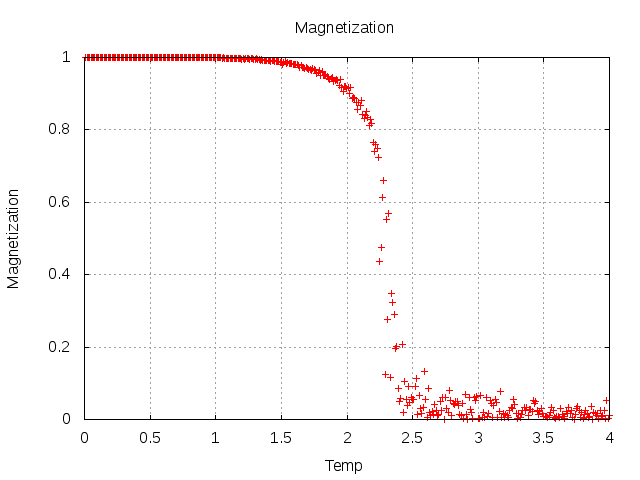
\includegraphics[width=0.75\textwidth]{MagVsT.png}
    %    \end{subfigure}
\end{figure}
\subsection{Magnetic Susceptibility}
\begin{figure}[H]
        \centering
        \caption{Magnetic Susceptibility vs Temperature \label{fig:chivsT}}
    %    \begin{subfigure}[b]{\textwidth}
                \centering
                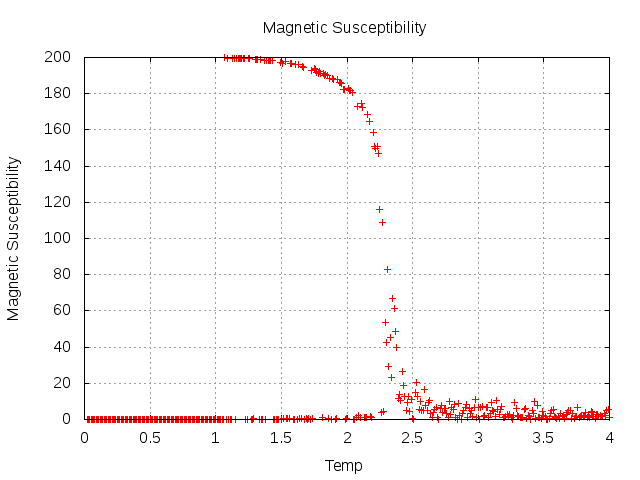
\includegraphics[width=0.75\textwidth]{chiVsT.png}
    %    \end{subfigure}
\end{figure}
It can be noted that the tail on top of the graph comes from the inaccuracy of the system but this disappears closer to the critical temperature. The averaging over all runs can solve this. 
\subsection{Critical Temperature}
It was found, looking at the data produced for the Magnetic Susceptibility that the critical temperature is $2.35$.
\subsection{Internal Energy}
\begin{figure}[H]
        \centering
        \caption{Internal Energy vs Temperature \label{fig:EvsT}}
    %    \begin{subfigure}[b]{\textwidth}
                \centering
                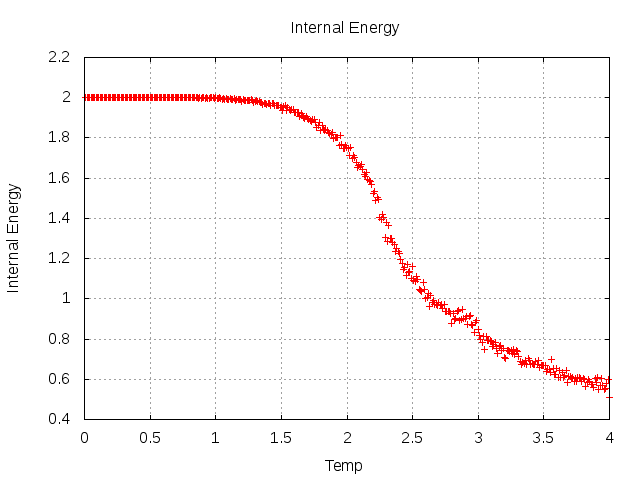
\includegraphics[width=0.75\textwidth]{EVsT.png}
    %    \end{subfigure}
\end{figure}
\subsection{Heat Capacity}
\begin{figure}[H]
        \centering
        \caption{Heat Capacity vs Temperature \label{fig:CvsT}}
    %    \begin{subfigure}[b]{\textwidth}
                \centering
                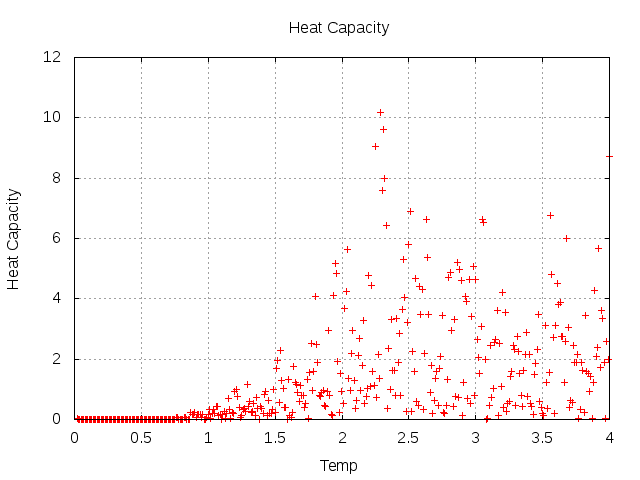
\includegraphics[width=0.75\textwidth]{C_vVsT.png}
    %    \end{subfigure}
\end{figure}
Heat capacity is difficult to obtain in the system created. This is due to the limited size of the system. Notice right at the critical temperature, there is an envelope signifying a peak, representing the rapid change in energy about this point.
\subsection{Critical Exponents}
\begin{figure}[H]
        \centering
        \caption{log(Magnetic Susceptibility) vs log(Temperature-Critical) \label{fig:logchivslogT}}
    %    \begin{subfigure}[b]{\textwidth}
                \centering
                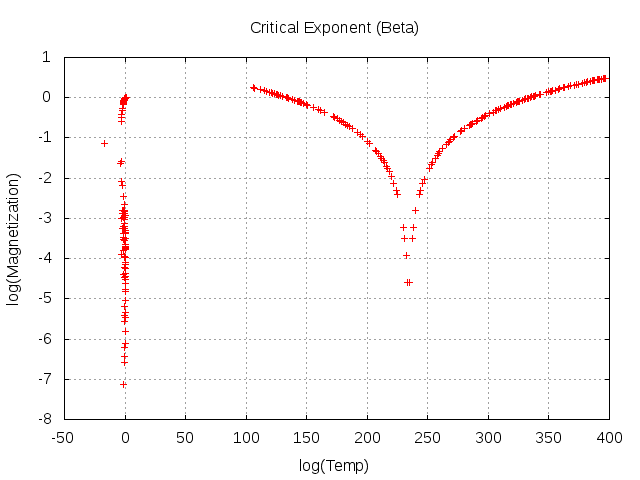
\includegraphics[width=0.75\textwidth]{Beta.png}
    %    \end{subfigure}
\end{figure}
\begin{figure}[H]
        \centering
        \caption{log(Heat Capacity) vs log(Temperature-Critical) \label{fig:logCvslogT}}
    %    \begin{subfigure}[b]{\textwidth}
                \centering
                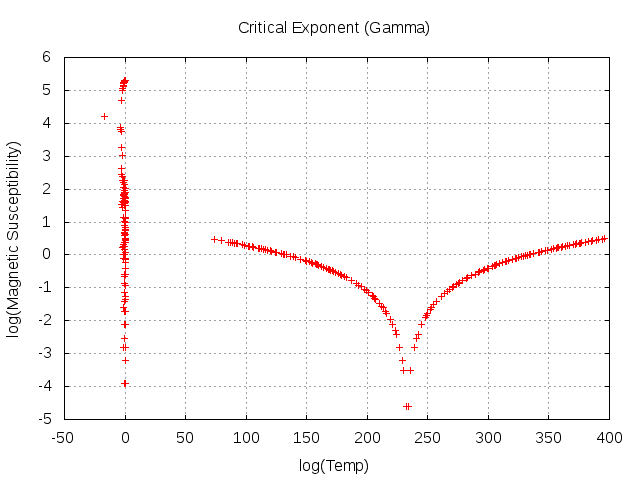
\includegraphics[width=0.75\textwidth]{Gamma.png}
    %    \end{subfigure}
\end{figure}


\newpage
\thispagestyle{empty}
\mbox{}

\newpage
\section{References}
\begin{thebibliography}{99}
\bibitem{JM} Thijssen, J. M. \textit{Computational Physics}. Ch. 8. Cambridge University Press. 1999. Print.
\end{thebibliography}

\end{document}
